% Realizar el mismo ejemplo en ambos y comparar mejoras, deficiencias de cada uno, diferencias..

\chapter{Estándares de Consulta de Información Geográfica y GeoSPARQL}
\label{ch:ge}

\begin{quote}
  {\bf\textsc{Resumen:}} Este capítulo define la arquitectura común que presentan las geometrías de características simples, estándar definido por OGC, y en el cual se basa el lenguaje de consulta geoespacial GeoSPARQL que vamos a usar en la prueba de concepto. Los conocimientos expuestos en este capítulo hacen referencia al nexo de unión existente entre las áreas de SIG y Web Semántica.
\end{quote}

\section{Estándares para la Información Geográfica y GeoSPARQL}

Uno de los objetivos del presente trabajo es estudiar las herramientas de la Web Semántica que se pueden utilizar para representar e incorporar Información Geográfica. Para ello es necesario conocer el nexo de unión que guardan ambos ámbitos aquí expuestos, puesto que al crear y desarrollar la ontología geoespacial GEOARES es necesario prestar especial atención a los estándares definidos por OGC, para su adecuada definición.


\subsection{Estándar OGC para la Información Geográfica}

El estándar expuesto en este apartado establece una arquitectura común y define los términos a usar dentro de dicha arquitectura para la representación geográfica y nivel lógico. La representación geográfica que vamos a usar se basa en el estándar \textit{ANSI/ISO SQL} y \textit{SQL/MM Part 3: Spatial}, definido por el organismo OGC, que contiene: jerarquía de clases y funciones estándar para datos espaciales en SQL \cite{AsignaturaSIG}.\\

En la figura \ref{fig:the-clases-geometry} se presenta la jerarquía de clases para geometrías de características simples, y como se observa es la misma que la mostrada en la figura \ref{fig:the-classes-of-geometries-in-wkt-figure-from-4} para la codificación WKT, vista en el \texttt{Capítulo 2}.

\begin{figure}[H]
	\centering
	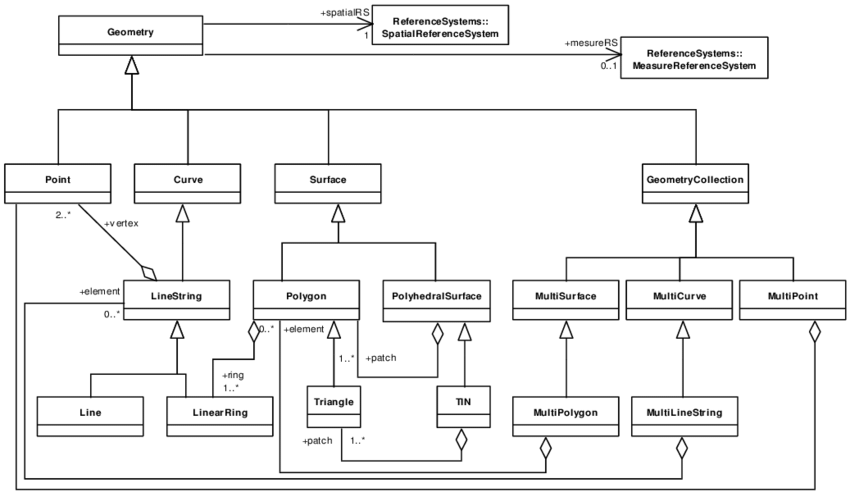
\includegraphics[width=1\linewidth]{imagenes/capitulo4/The-classes-of-geometries-in-WKT-figure-from-4}
	\caption{Jerarquía de clases \cite{estandar}}
	\label{fig:the-clases-geometry}
\end{figure}

Entonces, la figura \ref{fig:the-clases-geometry} muestra el modelo de objetos para la geometría de entidad simple usando la notación UML. La clase de \textit{Geometry} tiene subclases para \textit{Point}, \textit{Curve}, \textit{Surface} y \textit{GeometryCollection}, en donde cada objeto geométrico está asociado a un sistema de referencia espacial, que describe el espacio de coordenadas en el que se define el objeto geométrico \cite{estandar}. Para comprender mejor las clases representadas, vamos a ver una pequeña definición de cada una de ellas \cite{wkt-database} (figura \ref{fig:ejemplos}):

% La Figura 1 se basa en un modelo de Geometría extendida con clases especializadas de colección de 0, 1 y 2 dimensiones llamadas MultiPoint, MultiLineString y MultiPolygon para modelar geometrías correspondientes a colecciones de Puntos, LineStrings y Polígonos, respectivamente. MultiCurve y MultiSurface se presentan como superclases que generalizan las interfaces de colección para manejar Curvas y Superficies. La Figura 1 muestra líneas de agregación entre las clases de recolección de hojas y sus clases de elementos; Las líneas de agregación para las clases que no son de recolección de hojas se describen en el texto. Las colecciones no homogéneas son instancias de GeometryCollection.

\begin{itemize}
	\item \textit{\textbf{Point}}: representa una ubicación única en el espacio de coordenadas, tiene valores de coordenadas $x$ e $y$.
	
	\item \textit{\textbf{Curve}}: es una geometría unidimensional. 
	
	\item \textit{\textbf{LineString}}: es un subtipo de la clase \textit{Curve}, no tiene intersecciones propias y es cerrada si su punto de inicio es igual a su punto final.
	
	\item \textit{\textbf{Line}}: \textit{LineString} con exactamente dos puntos. 
	
	\item \textit{\textbf{LinearRing}}: \textit{LineString} cerrada y simple. 
	
	\item \textit{\textbf{Surface}}: es una geometría bidimensional (p.e. polígono con agujeros).% Esta clase es abstracta. %(es decir, no puede ser instanciada). %Una superficie simple puede consistir en un solo "parche" que tiene un límite "exterior" y 0 o más límites "interiores" (por ejemplo, un polígono con agujeros) .
	
	\item \textbf{Polygon}: \textit{Surface} simple plana que tiene exactamente un límite exterior y puede tener varios límites interiores que no se cruzan. %Cada polígono está topológicamente cerrado y no se cruzan dos límites. 
	
	\item \textit{\textbf{Triangle}}: es un \textit{Polygon} con 3 vértices distintos no colineales y sin límite interior. 
	
	\item \textbf{\textit{Polyhedral Surface}}: es una colección contigua de \textit{Polygon} que comparten segmentos límite comunes. %Cada par de polígonos que tocan tienen un límite común que se expresa como una colección finita de cadenas de líneas. 
	
	\item \textit{\textbf{Triangulated Irregular Network}}: un conjunto de puntos de triangulación para representar superficies en 3D.
	
	\item \textit{\textbf{Geometry Collection}}:  es un conjunto de geometrías distintas. 
		
	\item \textit{\textbf{MultiPoint}}: esta es una colección de geometría cuyos elementos son \textit{Point} que no están conectados.
	
	\item \textit{\textbf{MultiCurve}}: es una colección de geometría con elementos son \textit{Curve}.
	
	\item \textit{\textbf{MultiLineString}}: es una colección de geometría cuyos elementos son \textit{LineString}. 
	
	\item \textit{\textbf{MultiSurface}}: es una colección de geometría bidimensional cuyos elementos son \textit{Surface}.  
	
	\item \textit{\textbf{MultiPolygon}}: es una colección de superficies múltiples cuyos elementos son polígonos. Los límites de cada polígono pueden no cruzarse.
	
\end{itemize}

\begin{figure}[H]
	\centering
	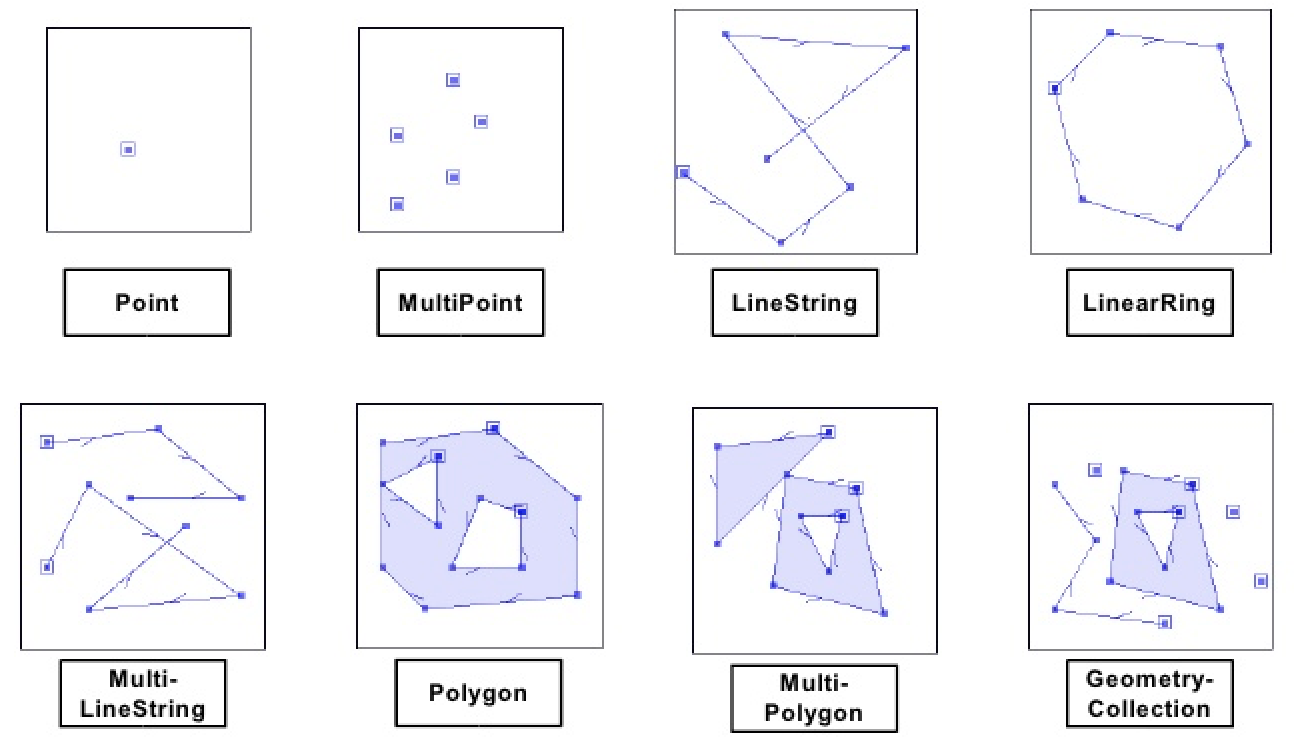
\includegraphics[width=0.9\linewidth]{imagenes/capitulo4/ejemplos}
	\caption{\textit{OpenGIS Simple Features Access} \cite{imagen-ejemplos}}
	\label{fig:ejemplos}
\end{figure}

Una vez que hemos definido las clases que componen el estándar, es necesario conocer las operaciones para las relaciones espaciales de la clase \textit{Geometry} (figura \ref{fig:geometry-class}).

\begin{figure}[H]
	\centering
	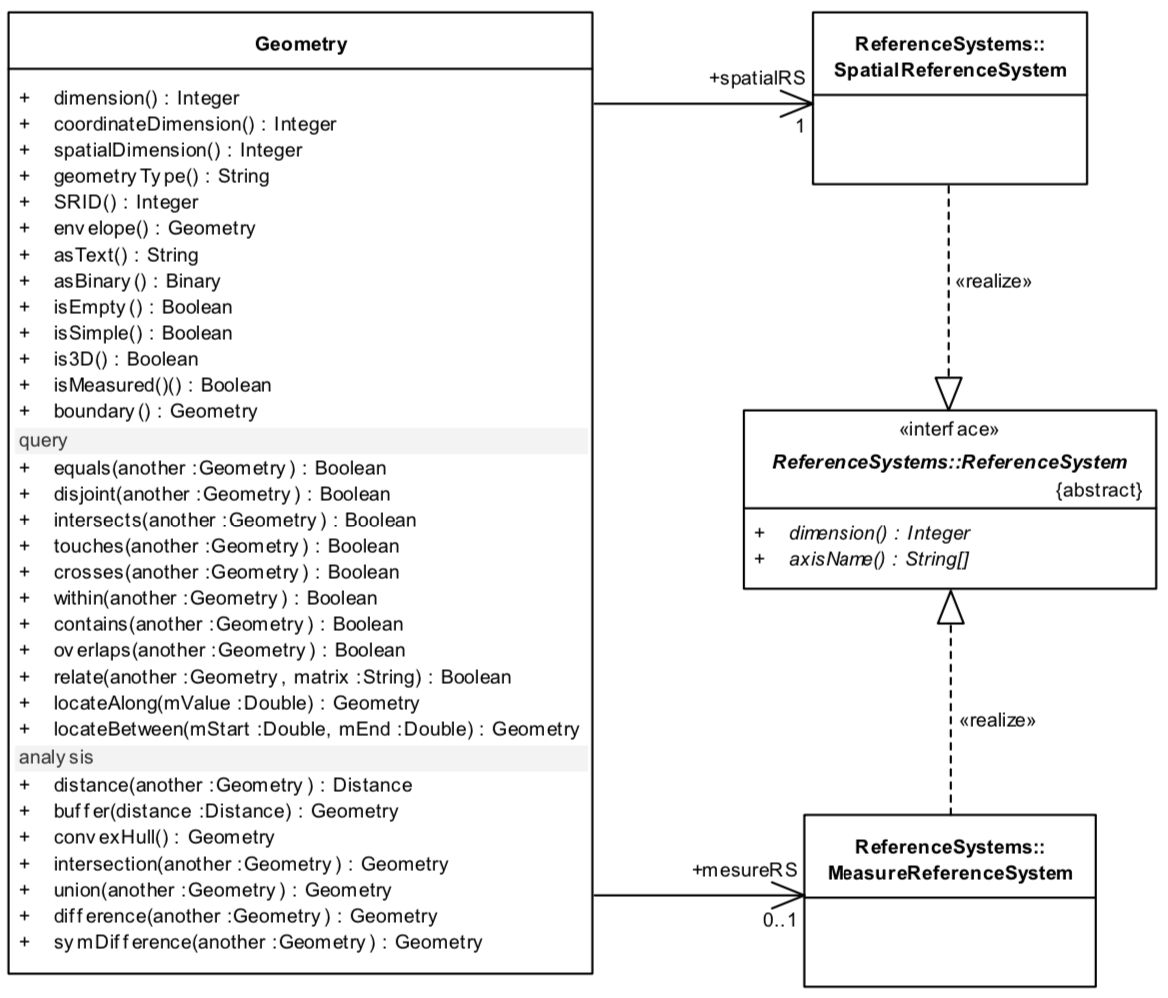
\includegraphics[width=1\linewidth]{imagenes/capitulo4/geometry-class}
	\caption{Operaciones de la clase \textit{Geometry} \cite{estandar}}
	\label{fig:geometry-class}
\end{figure}

\subsubsection{Operadores Booleanos de relaciones espaciales}

Comecemos por los \textbf{métodos para probar las relaciones espaciales entre objetos geométricos} de la clase \textit{Geometry}. Para cada uno de los métodos de la tabla \ref{estandar-funciones}), el tipo de retorno es entero, pero se interpreta como booleano, VERDADERO = 1, FALSO = 0. Corresponde a la parte de \texttt{query} de la figura \ref{fig:geometry-class} \cite{estandar, wkt-database}.



\subsubsection{Métodos de apoyo al análisis espacial}

Por otro lado los \textbf{métodos que apoyan el análisis espacial} de la clase \textit{Geometry} son análisis geométricos que dependen de la precisión de las representaciones de coordenadas y las limitaciones de la interpolación lineal en este estándar. La precisión del resultado a un buen nivel estará limitada por estos y otros problemas relacionados (tabla \ref{estandar-metodos}). Corresponde a la parte de \texttt{analysis} de la figura \ref{fig:geometry-class} \cite{estandar}.
 

 
 \begin{table}[H]
 	\caption{Operadores Booleanos de relaciones espaciales}
 	\label{estandar-funciones}
 	\centering
 	\begin{tabular}{|l|m{9.5cm}|}
 		\hline
 		\rowcolor[HTML]{EFEFEF} 
 		{\textbf{OPERADOR}} & { \textbf{DESCRIPCIÓN}} \\ \hline
 		\texttt{Equals}	&    \texttt{(anotherGeometry: Geometry): Integer} - Devuelve 1 (VERDADERO) si este objeto geométrico es ``espacialmente igual'' a otra \textit{Geometry}        \\ \hline
 		\texttt{Disjoint}	&       \texttt{(anotherGeometry: Geometry): Integer} - Devuelve 1 (VERDADERO) si este objeto geométrico es ``espacialmente disjunto'' de otra \textit{Geometry}              \\ \hline
 		\texttt{Intersects}	&   \texttt{(anotherGeometry: Geometry): Integer} - Devuelve 1 (VERDADERO) si este objeto geométrico ``se cruza espacialmente'' con otra \textit{Geometry}        \\ \hline
 		\texttt{Touches} &     \texttt{(anotherGeometry: Geometry): Integer} - Devuelve 1 (VERDADERO) si este objeto geométrico ``toca espacialmente'' otra \textit{Geometry}   (figura \ref{fig:touches})     \\ \hline
 		\texttt{Within}	&    \texttt{(anotherGeometry: Geometry): Integer} - Devuelve 1 (VERDADERO) si este objeto geométrico está ``espacialmente dentro'' de otra \textit{Geometry} (figura \ref{fig:within})               \\ \hline
 		\texttt{Contains} &     \texttt{(anotherGeometry: Geometry): Integer} -  Devuelve 1 (VERDADERO) si este objeto geométrico ``contiene espacialmente'' otra \textit{Geometry}      \\ \hline
 		\texttt{Overlaps}	&     \texttt{(anotherGeometry: Geometry): Integer} - Devuelve 1 (VERDADERO) si este objeto geométrico ``se superpone espacialmente'' a otra \textit{Geometry}         \\ \hline
 		\texttt{Crosses} &    \texttt{(anotherGeometry: Geometry): Integer} - Devuelve 1 (VERDADERO) si este objeto geométrico ``cruza espacialmente'' otra \textit{Geometry}    \\ \hline	
 		%\texttt{Relate} &   Devuelve 1 (VERDADERO) si este objeto geométrico está espacialmente relacionado con otra \textit{Geometry} probando las intersecciones entre el interior, el límite y el exterior de los dos objetos geométricos       \\ \hline	
 	\end{tabular}
 \end{table}

 \begin{figure}[H]
	\centering
	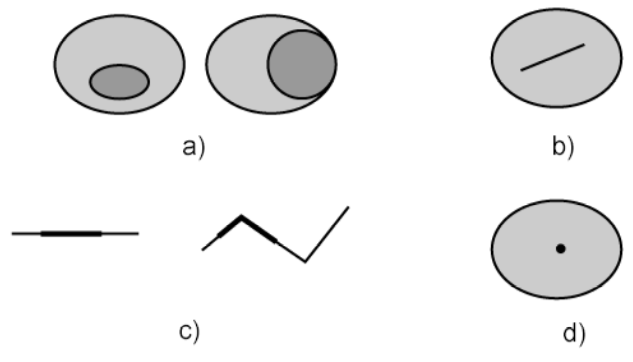
\includegraphics[width=0.7\linewidth]{imagenes/capitulo4/within}
	\caption{Ejemplos del operador \textit{Within} \cite{estandar}}
	\label{fig:within}
\end{figure}

 \begin{figure}[H]
 	\centering
 	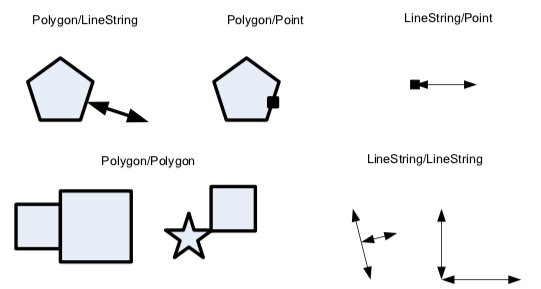
\includegraphics[width=0.71\linewidth]{imagenes/capitulo4/touches1}
 	\caption{Ejemplos del operador \textit{Touches} \cite{estandar}}
 	\label{fig:touches}
 \end{figure}


\begin{table}[H]
	\caption{Métodos de apoyo al análisis espacial}
	\label{estandar-metodos}
	\centering
	\begin{tabular}{|l|m{8.6cm}|}
		\hline
		\rowcolor[HTML]{EFEFEF} 
		{\textbf{FUNCIÓN} } & {\textbf{DESCRIPCIÓN}} \\ \hline
		\texttt{Distance}		&     \texttt{(anotherGeometry: Geometry):Double} - Devuelve la distancia más corta entre dos puntos de dos objetos geométricos        \\ \hline
		\texttt{Buffer} &     \texttt{(distance: Double): Geometry} -    Devuelve un objeto geométrico que representa todos los puntos cuya distancia desde este objeto geométrico es menor o igual que la distancia (figura \ref{fig:ejemplos-metodos} a)            \\ \hline
		\texttt{ConvexHull}	& \texttt{( ): Geometry} -     Devuelve un objeto geométrico que representa el casco convexo de este objeto geométrico (figura \ref{fig:ejemplos-metodos} b)             \\ \hline
		\texttt{Intersection} &   \texttt{(anotherGeometry: Geometry): Geometry} -    Devuelve un objeto geométrico que representa la intersección del conjunto de puntos de este objeto geométrico con otra \textit{Geometry}            \\ \hline
		\texttt{Union}	&  \texttt{(anotherGeometry: Geometry): Geometry}	-    Devuelve un objeto geométrico que representa la unión del conjunto de puntos de este objeto geométrico con otra \textit{Geometry}              \\ \hline
		\texttt{Difference} &  \texttt{(anotherGeometry: Geometry): Geometry } -  Devuelve un objeto geométrico que representa la diferencia de conjunto de puntos de este objeto geométrico con otra \textit{Geometry}            \\ \hline
		\texttt{SymDifference}	&   \texttt{(anotherGeometry: Geometry): Geometry}  - Devuelve un objeto geométrico que representa la diferencia simétrica del conjunto de puntos de este objeto geométrico con otra \textit{Geometry}                 \\ \hline
	\end{tabular}
\end{table}

\begin{figure}[H]
	\centering
	\begin{subfigure}[h]{0.32\textwidth} 
		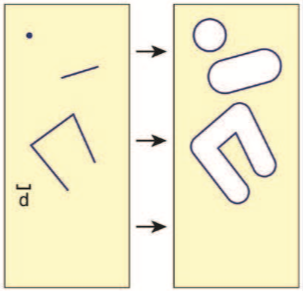
\includegraphics[width=\textwidth]{imagenes/capitulo4/buffer}
		\caption{\textit{Buffer}}
	\end{subfigure}       
	\begin{subfigure}[h]{0.32\textwidth} 
		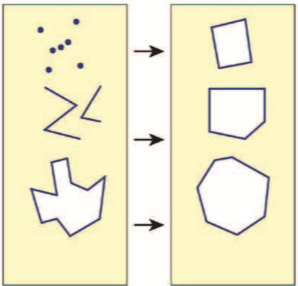
\includegraphics[width=\textwidth]{imagenes/capitulo4/convexHull}
		\caption{\textit{ConvexHull}}
	\end{subfigure}
	\caption{Ejemplos de los métodos \cite{AsignaturaSIG}}
	\label{fig:ejemplos-metodos}
\end{figure}



 


Con esto acabamos de definir los métodos y las funciones para manejar las subclases de las clases de \textit{Geometry}. A continuación, vamos a definir GeoSPARQL, lenguaje de consulta geoespacial muy relacionado con el estándar aquí expuesto.

\subsection{GeoSPARQL}

% tesis
% libro
\textbf{GeoSPARQL} es un estándar establecido por \textit{Open Geoespatial Consortium} (OGC). Es un lenguaje de consulta basado en SPARQL para recuperar información geoespacial de conjuntos de datos RDF en la Web Semántica \cite{libro-gis}. GeoSPARQL define gran parte de lo que se requiere para un lenguaje de consulta de este tipo al proporcionar vocabulario (clases, propiedades y funciones) que se pueden utilizar en gráficos RDF y consultas SPARQL para representar y consultar datos geoespaciales (figura \ref{fig:geosparql}). GeoSPARQL sigue el diseño modular típico de los estándares OGC \cite{ogc-geo, wkt-database}.

%Entre sus características podemos encontrar \cite{ogc-geo}: 
%\begin{itemize}
%	\item Vocabulario RDF/OWL para representar información geoespacial.
%	\item Funciones extensión a SPARQL para cálculos espaciales.
%	\item Conjunto básico de clases, propiedades y tipo de datos que son utilizados para construir patrones de consulta (figura \ref{fig:geosparql}). 
%\end{itemize}

\begin{figure}[H]
	\centering
	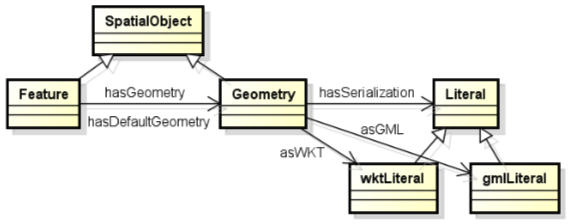
\includegraphics[width=0.9\linewidth]{imagenes/capitulo3/geosparql}
	\caption{Clases y propiedades básicas de GeoSPARQL \cite{tesis-otro}}
	\label{fig:geosparql}
\end{figure}

GeoSPARQL no define un vocabulario completo para representar información espacial, sino que define un conjunto central de clases, propiedades y tipos de datos que se pueden utilizar para construir patrones de consulta (figura \ref{fig:geosparql}) \cite{ogc-geo}. Es un lenguaje muy enfocado para la comunidad SIG. Por otro lado, para poder hacer uso de este tipo de consultas es necesario aplicar las especificaciones del estándar que vienen descritas en la documentación oficial\footnote{\url{https://www.opengeospatial.org/standards/geosparql}}. En la tabla \ref{topo-geosparql} podemos encontrar sus relaciones topológicas, mientras que en la tabla \ref{funciones-geosparql} podemos encontrar funciones de GeoSPARQL que incluyen alternativas de todas las propiedades de relación topológica, aplicadas como funciones en literales de geometría \cite{tesis-otro}. \\

Una decisión de diseño crucial de GeoSPARQL es usar valores literales para codificar geometrías como una sola unidad (puntos, líneas y polígonos,) e introducir dos tipos de datos RDF \texttt{geo:wktLiteral} y \texttt{geo:gmlLiteral} para estos literales. Dicha extensión está parametrizada por el estándar de serialización de OGC para codificar literales de geometría (WKT o GML). En nuestro caso, como ya hemos ido comentando vamos hacer uso del literal  \texttt{geo:wktLiteral}. \texttt{wktLiteral} consiste en un URI opcional que identifica el sistema de referencia de coordenadas seguido de la codificación WKT de una geometría, por ejemplo \cite{wkt-database}: 

\begin{lstlisting}
# Primera manera para representar el literal wktLiteral
"POINT(-83.38 33.95)"^^geo:wktLiteral

# Segunda manear para representar el literal wktLiteral
"<http://www.opengis.net/def/crs/EPSG/0/4326>
POINT(33.95 -83.38)"^^geo:wktLiteral
\end{lstlisting}

%Respecto la geometría permite puntos, líneas y polígonos, como vimos en el capítulo anterior y además la representación de la geometría debe de estar codificada en formato WKT 

\begin{table}[H]
	\caption{Relaciones topológicas con sus significados}
	\label{topo-geosparql}
	\centering
	\begin{tabular}{|l|l|}
		\hline
		\rowcolor[HTML]{EFEFEF} 
		{\textbf{OBJETO}} & { \textbf{DESCRIPCIÓN}} \\ \hline
		\texttt{sfEquals}	&              Espacialmente igual           \\ \hline
		\texttt{sfDisjoint}	&        Disjunto (no puede tocar)                 \\ \hline
		\texttt{sfIntersects}	&     Comparten al menos un punto                    \\ \hline
		\texttt{sfTouches} &          Se tocan externamente               \\ \hline
		\texttt{sfWithin}	&      Está dentro (puede tocar el límite)                   \\ \hline
		\texttt{sfContains} &             El inverso de \texttt{sfWithin}            \\ \hline
		\texttt{sfOverlaps}	&            Tienen algunos puntos comunes, misma dimensión             \\ \hline
		\texttt{sfCrosses} &         Por ejemplo, área cruza la línea                \\ \hline		
	\end{tabular}
\end{table}


También se definen propiedades para representar metadatos de geometrías (por ejemplo, \textit{geo:dimension} que captura la dimensión topológica) o para asociar geometrías con sus literales (\textit{geo:asWKT}). Además, esta extensión define funciones para realizar operaciones no topológicas en geometrías (por ejemplo, \textit{geof:distancie} o \textit{geof:ConvexHull}), las cuales son las mismas definidas anteriormente por el estándar \cite{wkt-database}.


\begin{table}[H]
	\caption{Funciones para comparar y manipular geometrías}
	\label{funciones-geosparql}
	\centering
	\begin{tabular}{|l|m{8.6cm}|}
		\hline
		\rowcolor[HTML]{EFEFEF} 
		{\textbf{FUNCIÓN} } & {\textbf{DESCRIPCIÓN}} \\ \hline
		\texttt{distance}		&       La distancia de dos literales geométricos medidos en unidades dadas                  \\ \hline
		\texttt{buffer} &           Literal de geometría como un literal de entrada con un buffer agregado, dado el radio y las unidades del buffer              \\ \hline
		\texttt{convexHull}	&      El casco convexo de un literal de geometría                   \\ \hline
		\texttt{intersection} &          La intersección de dos literales de geometría               \\ \hline
		\texttt{union}		&     Unión de dos literales de geometría                    \\ \hline
		\texttt{difference} &       La diferencia de dos literales de geometría                  \\ \hline
		\texttt{symDifference}	&      Establecer la diferencia simétrica de dos literales de geometría                  \\ \hline
		\texttt{envelope}  &              El cuadro delimitador de un literal de geometría           \\ \hline
		\texttt{boundary}		&    El límite de un literal de geometría                     \\ \hline
		\texttt{getsrid} &       URI del sistema de referencia espacial de un literal de geometría                  \\ \hline		
	\end{tabular}
\end{table}

En el apartado siguiente, haremos uso de este lenguaje para la obtención de la información geoespacial deseada, centrándonos en varios ejemplos prácticos, y su uso de cara al futuro.

\section{Conclusiones}

Este capítulo ha introducido el estándar usado en el lenguaje de consulta geoespacial GeoSPARQL, como nexo de unión de las áreas de los SIG y la Web Semántica. Se ha apreciado, que las funciones usadas en el GeoSPARQL son las mismas que OGC ha definido en su estándar. Con esto acabamos de comprobar como ha sido posible unir dos ámbitos que previamente parecían ser independientes el uno respecto del otro.